%%%%%%%%%%%%%%%%%%%%%%%%%%%%%%%%%%%%%%%%%
% Journal Article
% LaTeX Template
% Version 1.4 (15/5/16)
%
% This template has been downloaded from:
% http://www.LaTeXTemplates.com
%
% Original author:
% Frits Wenneker (http://www.howtotex.com) with extensive modifications by
% Vel (vel@LaTeXTemplates.com)
%
% License:
% CC BY-NC-SA 3.0 (http://creativecommons.org/licenses/by-nc-sa/3.0/)
%
%%%%%%%%%%%%%%%%%%%%%%%%%%%%%%%%%%%%%%%%%

%----------------------------------------------------------------------------------------
%	PACKAGES AND OTHER DOCUMENT CONFIGURATIONS
%----------------------------------------------------------------------------------------

\documentclass[10pt]{article} % Single column

%\documentclass[twoside,twocolumn]{article} % Two column

\usepackage{blindtext} % Package to generate dummy text throughout this template 

\usepackage[sc]{mathpazo} % Use the Palatino font
\usepackage[T1]{fontenc} % Use 8-bit encoding that has 256 glyphs
\linespread{1.05} % Line spacing - Palatino needs more space between lines
\usepackage{microtype} % Slightly tweak font spacing for aesthetics

\usepackage[spanish]{babel} % Language hyphenation and typographical rules

\usepackage{algorithm}
	
\usepackage[hmarginratio=1:1,top=32mm,columnsep=20pt]{geometry} % Document margins
\usepackage[hang, small,labelfont=bf,up,textfont=it,up]{caption} % Custom captions under/above floats in tables or figures
\usepackage{booktabs} % Horizontal rules in tables

\usepackage{lettrine} % The lettrine is the first enlarged letter at the beginning of the text

\usepackage{enumitem} % Customized lists
\setlist[itemize]{noitemsep} % Make itemize lists more compact

\usepackage{abstract} % Allows abstract customization
\renewcommand{\abstractnamefont}{\normalfont\bfseries} % Set the "Abstract" text to bold
\renewcommand{\abstracttextfont}{\normalfont\small\itshape} % Set the abstract itself to small italic text

\usepackage{titlesec} % Allows customization of titles
\renewcommand\thesection{\Roman{section}} % Roman numerals for the sections
\renewcommand\thesubsection{\roman{subsection}} % roman numerals for subsections
\titleformat{\section}[block]{\large\scshape\centering}{\thesection.}{1em}{} % Change the look of the section titles
\titleformat{\subsection}[block]{\large}{\thesubsection.}{1em}{} % Change the look of the section titles

\usepackage{fancyhdr} % Headers and footers
\pagestyle{fancy} % All pages have headers and footers
\fancyhead{} % Blank out the default header
\fancyfoot{} % Blank out the default footer
\fancyhead[C]{Dise\~no y An\'alisis de Algoritmos. \textbf{Proyecto \# 2: Tito el corrupto}} % Custom header text
\fancyfoot[RO,LE]{\thepage} % Custom footer text

\usepackage{titling} % Customizing the title section

\usepackage{hyperref} % For hyperlinks in the PDF

\usepackage{graphicx} % For images

\usepackage{pifont} % bullets

\usepackage{amsmath}

\usepackage{algpseudocode}

% Keywords command
\providecommand{\keywords}[1]
{
	\small	
	\vspace{0.5em}
	\noindent \textbf{\textit{Palabras clave --- }} #1
}


%----------------------------------------------------------------------------------------
%	TITLE SECTION
%----------------------------------------------------------------------------------------

\setlength{\droptitle}{-4\baselineskip} % Move the title up

\pretitle{\begin{center}\Huge\bfseries} % Article title formatting
	\posttitle{\end{center}} % Article title closing formatting
\title{\normalsize{Dise\~no y An\'alisis de Algoritmos }\\
	\Huge\bfseries Proyecto \# 2: Tito el corrupto \\
} % Article title
\author{% 
	
\includegraphics[width=15em]{logo.png} \vspace{1em}\\
	Laura Victoria Riera P\'erez\\
	Mari\'e del Valle Reyes \vspace{1em} \\
	\small Cuarto a\~no. Ciencias de la Computaci\'on. \\ % institution
	\small Facultad de Matem\'atica y Computaci\'on, Universidad de La Habana, Cuba \\ % institution
}
\date{\footnotesize \today } % Leave empty to omit a date


% Abstract configurations
\renewenvironment{abstract}
{\small
	\begin{center}
		\bfseries \abstractname\vspace{-.5em}\vspace{0pt}
	\end{center}
	\list{}{
		\setlength{\leftmargin}{1.5cm}%
		\setlength{\rightmargin}{\leftmargin}%
	}%
	\item\relax}
{\endlist}

\usepackage{amsthm}
\usepackage{amssymb}
\usepackage{todonotes} % \TODO
\usepackage{listings} % Code listings
\usepackage{xcolor}

\definecolor{backcolour}{rgb}{0.95,0.95,0.92}

\newcommand{\csl}[1]{\colorbox{backcolour}{\texttt{#1}}}

\newcommand{\imgcaption}[2]{\tiny \textbf{Figura #1.} #2.}

\newcommand{\mgc}[2][]{\colorbox{backcolour}{\texttt{\_\_#2\_\_#1}}}

\newcommand{\mgccapt}[1]{\texttt{\_\_#1\_\_}}

\newtheorem{thm}{Teorema}
\newtheorem{mydef}{Definici\'on}%[section]
\newtheorem{lem}{Lema}
\newtheorem{fig}{\scriptsize{Figura}}
\newtheorem{col}{Corolario}


\renewcommand{\qedsymbol}{\rule{0.7em}{0.7em}}

% Hyperlinks configurations
\hypersetup{
	colorlinks=true,
	linkcolor=black,
	filecolor=magenta,      
	urlcolor=cyan,
	pdftitle={Overleaf Example},
	pdfpagemode=FullScreen,
}

%----------------------------------------------------------------------------------------

\begin{document}
	% Print the title
	\maketitle
	
	%----------------------------------------------------------------------------------------
	%	ARTICLE CONTENTS
	%----------------------------------------------------------------------------------------
	
	\section{Repositorio del proyecto}
	
	\begin{center}
		\href{https://github.com/computer-science-crows/algorithms-design-and-analysis}{https://github.com/computer-science-crows/algorithms-design-and-analysis}
	\end{center}

	\section{Definici\'on inicial del problema} 

	Tito se dió cuenta de que la carrera de computación estaba acabando con él y un día decidió darle un cambio radical a su vida. Comenzó a estudiar Ingeniería Industrial. Luego de unos años de fiesta, logró finalmente conseguir su título de ingeniero. Luego de otros tantos años ejerciendo sus estudios, consiguió ponerse a la cabeza de un gran proyecto de construcción de carreteras.
	
	La zona en la que debe trabajar tiene $n$ ciudades con $m$ posibles carreteras a construir entre ellas. Cada ciudad que sea incluida en el proyecto aportará $a_i$ dólares al proyecto, mientras que cada carretera tiene un costo de $w_i$ dólares. Si una carretera se incluye en el proyecto, las ciudades unidas por esta también deben incluirse.
	
	El problema está en que Tito quiere utilizar una de las habilidades que aprendió en sus años de estudio, la de la malversación de fondos. Todo el dinero necesario para el proyecto que no sea un aporte de alguna ciudad, lo proveerá el país y pasará por manos de Tito. El dinero aportado por las ciudades no pasará por sus manos. Tito quiere maximizar la cantidad de dinero que pasa por él, para poder hacer su magia. Ayude a Tito a seleccionar el conjunto de carreteras a incluir en el proyecto para lograr su objetivo.
	

	\section{Definici\'on en t\'erminos matem\'atico - computacionales}\label{section_2}
	
	La entrada de nuestro problema es la cantidad de ciudades $n$, la cantidad de carreteras $m$, una lista $a$ con el dinero aportado por cada ciudad y una lista $w$ con cada carretera \todo{entre ciudades} y su costo. El objetivo es maximizar la diferencia de la suma de los costos de construir las carreteras seleccionadas y la suma del aporte de cada una de las ciudades que intervienen en esas carreteras. La salida del problema es la distribuci\'on del proyecto como dos listas, una que contiene las ciudades y otra las carreteras a construir tal que se obtenga la ganancia m\'axima.
	
	\subsection{Problema "Proyectos e Intrumentos''}
	
	Uno de los problemas de flujo más conocidos es el de "Proyectos e Instrumentos". En este, se tienen un conjunto de proyectos que podemos hacer, cada uno con su costo, y un conjunto de instrumentos, cada uno con algún costo tambi\'en. Cada proyecto depende de algunos instrumentos, y cada instrumento se puede utilizar cualquier número de veces. Se debe elegir un subconjunto de proyectos y un subconjunto de instrumentos tal que, si se elige un proyecto, también se elijan todos los instrumentos de los que depende este proyecto, y maximizar la diferencia entre la suma de los costos de los proyectos elegidos y la suma de los costes de los instrumentos elegidos.
	
	Como puede observarse, este es precisamente el problema que nos ocupa, siendo los proyectos, las carreteras y los intrumentos, las ciudades. Este se puede modelar mediante una red de flujo contruyendo un grafo dirigido $G = (V, E)$ como el que se describe a continuaci\'on:
	
%	Se construye un grafo dirigido $G'=(V',E')$, donde $|V'| = m + n + 2$ y $|E'|= 3 \cdot$ m + n. 
	\begin{itemize}
		\item El conjunto $V$ est\'a formado por $n+m+2$ v\'ertices que representan cada ciudad y cada carretera, adem\'as de un v\'ertice $s$ que representa la fuente y un v\'ertice $t$ que representa el receptor. 
		\item El conjunto $E$ est\'a formado por $n+3\cdot m $ arcos, distribuidos de la siguiente forma:
		\begin{itemize}
			\item Arcos desde $s$ hasta cada v\'ertice que representa una carretera con capacidad igual al valor $w_i$ dado de entrada, que representa el costo de construir la carretera $i$.
			
			\item Arcos desde cada v\'ertice que representa una ciudad hacia el v\'ertice $t$ con capacidad igual al valor $a_i$ que representa el aporte de la ciudad $i$ al ser incluida en el proyecto.
			
			\item Arcos desde cada v\'ertice que representa una carretera hacia cada v\'ertice ciudad que la conforma (extremos) con capacidad igual a $\infty$.
		\end{itemize}
	\end{itemize}
	
	\section{Soluciones implementadas}
	
	\subsection{Backtrack}
		Como primera solución al problema fue implementado un \textit{backtrack}. Esta es una solución correcta, ya que prueba todas las combinaciones de posibles carreteras y se queda con la que más ganancia aporte, pero muy ineficiente \textit{O($2^{m}$)}. En una computadora de 32GB de RAM, intel core i7-11na generación, se puede resolver para una cantidad máxima 5 ciudades con 5 aristas. Dicha solución puede ser encontrada en src/solutions/backtrack\_solution.py.
	
	\subsection{Soluci\'on utilizando flujo}
	
%	\subsubsection{Preliminares}
%	\begin{mydef}
%		Una \textbf{red de flujo} $G=(V,E)$ es un grafo dirigido en el que a cada par ordenado (u,v),  u, v$\in$V, se le asocia una función de capacidad no negativa c(u,v)$\geq$ 0 y en el que se distinguen dos vértices: la fuente s y el receptor t.
%	\end{mydef}
%
%	\begin{mydef}\label{red_flujo}
%		Sea G=〈V,E〉 una red de flujo con función de \textbf{capacidad} c y vértices fuente y receptor s y t respectivamente. Un \textbf{flujo} en G es una función real $f:V x V\rightarrow \mathbb{R}^+$ que satisface las siguientes propiedades:
%		
%		\begin{enumerate}
%			\item Restricci\'on de capacidad: Para todo u,v$\in$V se cumple que
%			\begin{equation}
%				0 \leq f(u,v) \leq c(u,v)
%			\end{equation}
%		
%			\item Conservaci\'on de flujo: Para todo u$\in$V- \{s,t\}, se cumple que
%			\begin{equation}
%				\sum_{v \in V} f(v,u) = \sum_{v \in V} f(u,v)
%			\end{equation}
%			
%		\end{enumerate}
%		
%	\end{mydef}
%
%	\begin{mydef}\label{flujo_neto}
%		A la cantidad  no negativa f(u,v) se le denomina \textbf{flujo neto} de u a v.
%	\end{mydef}
%
%	\begin{mydef}\label{valor_flujo}
%		El \textbf{valor de un flujo} se define como:
%		
%		\begin{equation}
%			|f|=\sum_{v \in V} f(s,v)
%		\end{equation}
%	\end{mydef}
%
%	\begin{mydef}\label{capacidad_residual}
%		Sea G=〈V,E〉 una red de flujo con origen s y receptor t. Sea f un flujo en G, y sean u,v $\in$ V.
%		
%		Se define la \textbf{capacidad residual} mediante la siguiente función:
%		
%		\begin{equation}
%			c_f(u,v) = 	\left\{		
%			\begin{array}{lr}				
%				c(u,v) -f(u,v) & , \text{si (u,v) $\in$ E}\\
%				f(v,u) &, \text{si (v,u) $\in$ E}\\
%				0 &,\text{en otro caso}\\
%			\end{array}
%		\right.
%		\end{equation}
%	
%	La \textbf{red residual} de G inducida por f es una red $G_f=(V,E_f)$, donde 
%	$E_f= \{ (u,v) \in VxV | c_f(u,v)>0 \}$.
%	\end{mydef}
%
%	\begin{mydef}\label{aumento_flujo}
%		
%		Si f es un flujo en la red original G y $f'$ es un flujo en la red residual correspondiente $G_f$, entonces, se define el aumento del flujo f (en la  red  original) por $f'$, y denotado por $f\uparrow f'$, a la función  $f\uparrow f'$: VxV$\rightarrow$ $\mathbb{R}$ dada por la expresión:
%		
%		\begin{equation}
%			f\uparrow f'(u,v) = \left\{ \begin{array}{lr}
%				f(u,v) + f'(u,v) - f'(v,u) & \text{si (u,v) $\in$ E}\\
%				0 & \text{en otro caso}\\
%			\end{array}
%		\right.
%		\end{equation}
%		
%	\end{mydef}
%	
%	\begin{lem}
%		|f $\uparrow$ f'|=|f|+|f'|
%	\end{lem}
%	
%	\begin{mydef}\label{camino_aumentativo}
%		Dada una red de flujo G=〈V,E〉 y un flujo f, un \textbf{camino aumentativo} p es un camino simple de s a t en la red residual $G_f$.
%	\end{mydef}
%
%	\begin{mydef}\label{capacidad_residual_c_a}
%		La capacidad residual de un camino aumentativo p, denotada por $c_f(p)$, es el valor máximo en el cual es posible aumentar el flujo en cada arista del camino sin violar la restricción de capacidad
%		\begin{equation}
%			c_f(p) = min\{c_f(u,v) | (u,v) \in p \}
%		\end{equation}
%	\end{mydef}
%
%	\begin{lem}\label{flujo_red_r}
%		Sea G=〈V,E〉 una red de flujo, sea f un flujo en G y sea p un camino aumentativo en $G_f$. Si se define el flujo $f_p$ , sobre la red residual, como
%		
%		\begin{equation}
%			f_p(u,v) = \left\{
%			\begin{array}{lr}
%				c_f(p) & \text{si (u,v) $\in$ p}\\
%				0 & \text{en otro caso}
%			\end{array}
%			\right.
%		\end{equation}
%		entonces el valor de $f_p$ es $|f_p|=c_f(p)>0$	
%		
%	\end{lem}
%
%	\begin{col}
%		Sea G=〈V,E〉 una red de flujo, sea f un flujo en G y sea p un camino aumentativo en $G_f$. Sea $f_p$ definida mediante la ecuación * y supóngase que se aumenta f por $f_p$. Entonces la función f $\uparrow$ $f_p$ es un flujo en G con valor |f $\uparrow$ $f_p$| = |f| + |$f_p$| > |f|.
%	\end{col}
%
%	\begin{mydef}\label{corte}
%		Un \textbf{corte} (S,T) de una red de flujo G = (V,E) es una partici\'on de V en dos conjuntos S y T = V-S de modo 	ue s $\in$ S y t $\in$ T.
%	\end{mydef}
%
%	\begin{mydef}\label{flujo_corte}
%		Si f es un flujo, entonces el \textbf{flujo neto} f(S,T) a trav\'es del corte (S,T) se define como
%		\begin{equation}
%			f(S,T) = \sum_{u\in S} \sum_{v\in T} f(u,v) - \sum_{u \in S}\sum_{v \in T} f(u,v)
%		\end{equation}
%	Adem\'as, la \textbf{capacidad} del corte (S,T) se define como
%	\begin{equation}
%		c(S,T) = \sum_{u \in S}\sum_{v \in T}c(u,v).
%	\end{equation} 
%	\end{mydef}
%
%	\begin{lem}
%		Sea f un flujo en una red de flujo G con origen s y receptor t. Sea (S,T) un corte cualquiera de G. Entonces el flujo neto a través del corte f(S,T) es igual al valor del flujo, osea, |f|
%		\begin{equation}
%			f(S,T) = |f|
%		\end{equation}
%	\end{lem}
%
%	\begin{col}
%		El valor de cualquier flujo en una red de flujo G está acotado superiormente por la capacidad de cualquier corte de G.
%		\begin{equation}
%			f(S,T) = |f| \leq c(S,T)
%		\end{equation}
%	\end{col}
%	
%	\begin{thm}
%		Si f es un flujo en una red de flujo G=〈V,E〉 con un origen s y un receptor t, entonces las siguientes condiciones son equivalentes:
%		\begin{enumerate}
%			\item f es un flujo máximo en G. 
%			\item En la red residual $G_f$ no se pueden encontrar más caminos aumentativos.
%			\item  |f|=c(S,T) para algún corte (S,T) de G.
%		\end{enumerate}
%	\end{thm}

%		\subsubsection{Algortimo Ford-Fulkerson}\label{ff}
%	
%	El algoritmo Ford-Fulkerson es utilizado para encontrar el flujo máximo en una red de flujo [\ref{red_flujo}]. Esta red se representa como un grafo dirigido donde cada arista tiene una capacidad que indica la cantidad máxima de flujo que puede pasar por ella.
%	
%	El algoritmo encuentra el flujo máximo en la red de flujo utilizando la técnica de aumentar caminos. En cada iteración del algoritmo, se busca un camino aumentativo [\ref{camino_aumentativo}], es decir, un camino desde el nodo fuente hasta el nodo receptor donde todas las aristas tienen capacidad positiva y suficiente para aumentar el flujo actual. Una vez encontrado el camino aumentativo, se aumenta el flujo en esa ruta tanto como sea posible. Este proceso se repite hasta que ya no haya caminos aumentativos en el grafo residual.
%	
%	El grafo residual se obtiene a partir del grafo original restando el flujo actual del flujo máximo para obtener la capacidad residual de cada arista. De esta manera, se pueden buscar caminos amentativos en el grafo residual sin utilizar aristas que ya están completamente saturadas.
%	
%	El algoritmo Ford-Fulkerson garantiza que, una vez que se alcanza el flujo máximo, no hay caminos aumentativos en el grafo residual y, por lo tanto, el flujo es óptimo.
	
	\subsubsection{Propuesta de soluci\'on}
	
	Se aplica un algoritmo de flujo sobre G y se toma el corte m\'inimo (S, T), construyendo la respuesta basada en este corte de la siguiente manera: 
	\begin{itemize}
		\item si un proyecto-vértice pertenece a S, entonces tomamos este proyecto;
		\item si un vértice-instrumento pertenece a S, entonces tomamos este instrumento; todos los demás proyectos e instrumentos se descartan. 
	\end{itemize}
	 
	 el valor del recorte es igual al costo total de los instrumentos tomados y los proyectos descartados, y debemos minimizarlo. Entonces, el corte mínimo en esta red denota la mejor respuesta.
	
	Correctitud

	Creando G' se puede modelar lo anterior usando un algoritmo de flujo, miraremos nuestro corte mínimo, si se corta algún arco entre 
	y algún 
	entonces se incluiría el uso de la ganancia de la arista asociada a 
	en G, si se corta algún arco entre la 
	y 
	, entonces se tiene que satisfacer la perdida del j-esimo vertice, se puede ver que si se incluye una arista de G entonces se tienen que incluir sus vertices asociados en G o sacar la arista de la solución pues sería imposible cortar el arco de peso 
	entre ellos en G'.
	
	Luego si no se satura alguna arista de G' desde 
	a 
	implicaría que no se puede satisfacer la perdida que genera por lo que el vertice de G asociado 
	no se debe incluir en la solución.
	
	Demostración de correctitud
	
	Sabemos que el valor del flujo es igual a la capacidad del corte mínimo y que las aristas que unen a los vértices que pertenecen a 
	con los vértices que pertenecen a 
	están saturadas.
	
	Sea 
	el corte mínimo.
	
	Si dado el corte mínimo existe un nodo carretera 
	tal que 
	esa carretera no será construida porque implica que el dinero que gana Tito al construir 
	es menor o igual que el dinero que aportan las ciudades que conecta y por tanto Tito no ganaría nada.
	
	Si dado el corte mínimo existe un nodo ciudad 
	que pertenece a 
	es necesario conectar esa ciudad, la artista entre 
	y 
	está saturada por el dinero de las carreteras, o sea, las calles que conectan a 
	aportan más dinero del que resta 
	.
	
	Por tanto la respuesta final será todo 
	tal que 
	.
	
	\subsubsection{Complejidad Temporal}
	
	La funci\'on principal es \textsc{corruption\_strategy(\textit{n, m, a, w})}. La funci\'on tiene como par\'ametros: $n$, el n\'umero de ciudades, $m$, el n\'umero de carreteras, $a$, lista con el aporte de cada ciudad, $w$, lista con el costo de cada carretera. El pseudoc\'odigo siguiente permite un acercamiento a la implementaci\'on realizada.
	
	\begin{algorithmic}[1]
		\Function{corruption\_strategy}{\textit{(n, m, a, w)}}
		
		\State $G$ = \textsc{build\_graph\textit{(n, m, a, w)}}
		\State $G_r$ =\textsc{ get\_min\_cut\_residual\_graph(\textit{G})}
		\State \textit{cities, roads, profit} = \textsc{get\_project\_distro(\textit{$G_r$, G})}
		
		\Return \textit{cities, roads, profit}
		\EndFunction
	\end{algorithmic}

	Para el trabajo con grafos por razones de comodidad se utilizó la librería networkx de Python.	En el cálculo de la complejidad temporal no se tiene en cuenta el costo de las operaciones sobre
	grafos creados con la librería anterior.
	
	En la l\'inea 2 del m\'etodo anterior, se llama a la funci\'on \textsc{build\_graph\textit{(n, m, a, w)}}, la cual se encarga de construir el grafo $G$ explicado en la secci\'on \ref{section_2}. La complejidad temporal de dicha funci\'on es $O(|V| + |E|)$, ya que por cada carretera se contruye una arista entre el nodo fuente y el nodo que representa a dicha carretera,  por cada par de ciudades que conforman una carretera, se crean dos arcos, cada una desde la carretera hasta las respectivas ciudades y tambi\'en, por cada nodo que representa a una ciudad, se contruye una arista con el nodo receptor.
	
	Una vez creado el grafo, se llama a la funci\'on \textsc{ get\_min\_cut\_residual\_graph(\textit{G})}, que tiene como par\'ametro el grafo $G$. El pseudoc\'odigo del m\'etodo se muestra a continuaci\'on.
	
	\begin{algorithm}[h]
		
		\algblock[TryCatchFinally]{try}{endtry}
		\algcblock[TryCatchFinally]{TryCatchFinally}{finally}{endtry}
		\algcblockdefx[TryCatchFinally]{TryCatchFinally}{catch}{endtry}
		[1]{\textbf{catch} #1}
		{\textbf{end try}}
		\begin{algorithmic}[1]
			\Function{get\_min\_cut\_residual\_graph}{$G$}
			\State $G_r$ = \textsc{get\_residual\_graph(\textit{G})}
			\State \textit{s} = \textit{'source'}
			\State \textit{t} = \textit{'sink'}
			
			\State \textit{p} = \textsc{find\_augmenting\_path(\textit{$G_r$, s, t})}
			
			\While {\textit{p != None}}
			\State \textit{capacity\_p} = \textsc{residual\_capacity\_path($G_r$, p)}
			\For{\textit{(u, v) in p}}
			\try
			\State \textit{G[u][v]['flow']} = \textit{G[u][v]['flow'] + capacity\_p}
			\catch
			\State \textit{G[v][u]['flow'] = G[v][u]['flow'] - capacity\_p}
			\endtry
			\State $G_r$ = \textsc{get\_residual\_graph($G$)}
			\State \textit{p} = \textsc{find\_augmenting\_path($G_r, s, t$)}
			\EndFor
			\EndWhile
			
			
			\Return $G_r$
			\EndFunction 
		\end{algorithmic}
	
	\end{algorithm}

	La funci\'on consiste en aplicar el algortimo Ford-Fulkerson al grafo $G$, por tanto tiene complejidad temporal $O(|E||f*|)$, donde $f*$ es el flujo m\'aximo calculado por el algoritmo. Primero, se construye el grafo residual de $G$,  $G_r$ (l\'inea 2), el cual se explica en la subsecci\'on \ref{ff}, y se encuentra un camino aumentativo $p$ en dicho grafo (l\'inea 5). El m\'etodo \textsc{get\_residual\_graph(\textit{G})}, tiene una complejidad temporal $O(|$E$|)$, ya que recorre todas los arcos de $G$ y construye $G_r$ con los mismos nodos de $V$, pero con los arcos de $E$ cuya capacidad es mayor que su flujo. La funci\'on \textsc{find\_augmenting\_path(\textit{$G_r$, s, t})} realiza un DFS por tanto tiene complejida temporal $O(|V| + |E_r|)$, donde $E_r$ son el conjunto de arcos del grafo residual $G_r$. Luego, se continua actualizando el grafo residual cada vez que se encuentra un camino aumentativo. El ciclo termina cuando no exista camino aumentativo en la red residual. Este m\'etodo retorna el grafo residual resultante al hallar el flujo m\'aximo.
	
	Despu\'es de aplicar el algoritmo de flujo a $G$, se obtiene el \'ultimo $G_r$ y a este grafo se le aplica el m\'etodo \textsc{get\_project\_distro(\textit{$G_r$, G})} que halla el corte m\'inimo $(S,T)$ y determina las ciudades, carreteras y el valor de la ganancia que es la soluci\'on del problema, a partir de los nodos que conforman la partici\'on S. Este m\'etodo tiene complejidad temporal $O(|S|)$.
	
	En conclusi\'on, la funci\'on \textsc{corruption\_strategy(\textit{n, m, a, w})} tiene complejidad temporal,
	
	\begin{equation}
		\begin{aligned}
			O(|V| + |E| + |E||f*| + |S|) &=\text{ m\'ax}\{|V|, |E|, |E||f*|, |S|\}\\
			&=O(|E||f*|)\\
		\end{aligned}		
	\end{equation}
	ya que $|V|$ < $|E|$, por la forma en que est\'a constru\'ido $G$ y $|S|<|V|$, debido a que al menos el nodo receptor $t$ no pertenece a $S$.

	

	\subsubsection{Complejidad Espacial}
	
	La complejidad espacial de nuestra implementaci\'on es $O(2n + 4m)$. El algoritmo utiliza como entrada una lista de tama\~no $n$ y otra de tama\~no $m$ como se explic\'o en la definici\'on del problema. Adem\'as, se crea un grafo dirigido con la librer\'ia networkx de Python que tiene $2 + m + n$ v\'ertices y $n + 3m$ aristas, cuyo costo asumimos no es mayor que $O(2n + 4m)$.
		
	\section{Generador de casos de prueba}
	
	En \textit{src/app/generator.py} fue implementado un generador, el cual recibe una cantidad $ s $ de muestras a producir, genera valores random con el formato de entrada de los algoritmos implementados, halla la soluci\'on \'optima con $ backtrack $ y las guarda en $ json/test\_cases.json $. Se generaron 3000 casos de prueba.
	
	\section{Tester}
	En \textit{src/app/tester.py} fue implementado un tester, que recibe una funci\'on y prueba el desempe\~no de la misma en cuanto a si obtuvo la soluci\'on \'optima o no, y el tiempo que demor\'o en hacerlo, comparando con los casos de prueba obtenidos con el generador. Adem\'as, estos resultados se guardan en un $ .json $ con el nombre de la funci\'on en la carpeta tests. La soluci\'on implementada fue testeada para todos los casos de prueba generados y puede encontrarse en $ json/tests/corruption\_strategy\_solution.json $ .
	
	\section{Comparaci\'on de soluciones implementadas}          

    A continuaci\'on se muestra una gr\'afica por cada algoritmo con el tiempo que demor\'o en cada uno de los 3000 tests. Como podemos observar, en los casos analizados, el \textit{backtrack} puede demorar desde 0.000 hasta 0.016 segundos en ejecutarse, pero la mayor\'ia de los casos oscilan entre 0.000 y 0.002. La \textit{soluci\'on con flujo} para todos los casos se demora menos de 0.0016 segundos, lo cual lo convierte en una soluci\'on significativamente mejor que el backtrack.
    
    \begin{center}
    	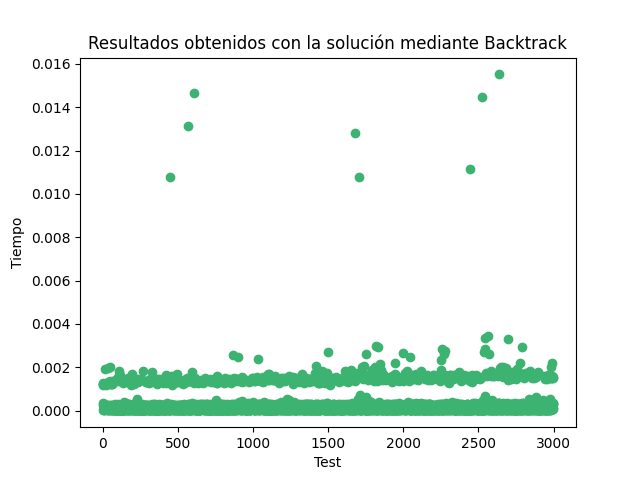
\includegraphics[width=7cm]{Backtrack_results.png}
    	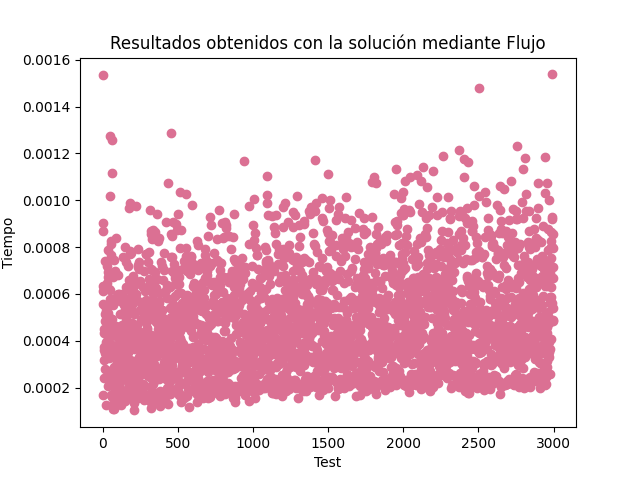
\includegraphics[width=7cm]{Flujo_results.png}
    \end{center}  
    
    Adem\'as, en la siguiente gr\'afica se ofrece una comparaci\'on del tiempo promedio que le toma a cada algoritmo ejecutar los casos de prueba. 
    
    \begin{center}
    	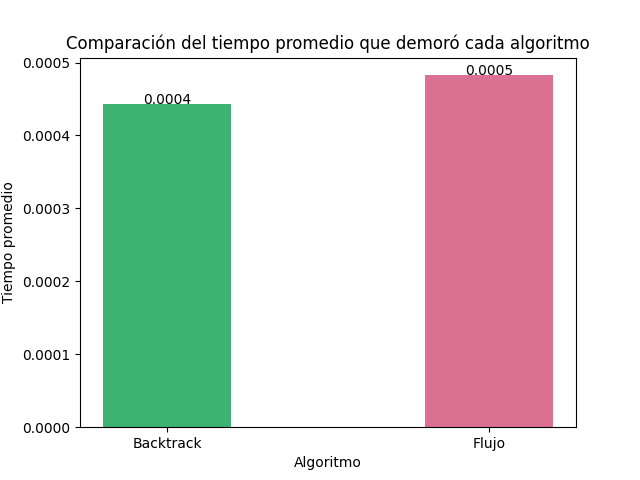
\includegraphics[width=7cm]{Bar_comparative_plot.png}
    \end{center}
	
	\todo{chequear gr\'aficas}
	\begin{center}
		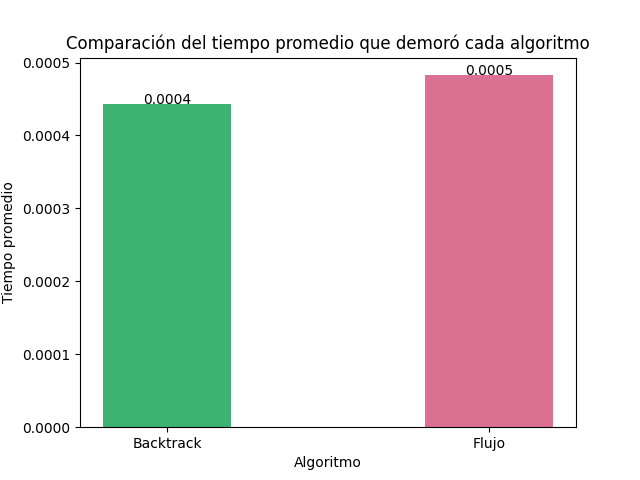
\includegraphics[width=7cm]{Bar_comparative_plot.png}
	\end{center}
	
	\begin{thebibliography}
		a
		\bibitem{introduction} Cormen, Thomas H. y otros. \emph{Introduction to Algorithms}. 
		The MIT Press.
		4ta Edici\'on.		
		Cambridge, Massachusetts.
		2022.
	\end{thebibliography}
\end{document}


